% BEGIN PREAMBEL
\documentclass[9pt, xcolor=dvipsnames, table]{beamer}
\usepackage[british]{babel}

\usepackage{xcolor}
\usepackage{multimedia}
\usepackage{amsmath,amsfonts,amssymb}
\usepackage{upgreek}
\usepackage[version=3]{mhchem}
\usepackage{lmodern}
\usepackage{graphicx}
\usepackage{multicol}
\usepackage{color}
\usepackage{tabularx}
\usepackage{pgfpages}
\usepackage{fontawesome}
\usepackage{wrapfig}
\usepackage{siunitx}
\usepackage{fontspec}
\usepackage{tikz}
\usepackage{textpos}
\usepackage{booktabs}
\usepackage{caption}
\usepackage{subcaption}
\usepackage{wasysym}
\usepackage{animate}
\usepackage{xparse}
\usepackage{pifont}
\usepackage{xfrac}
\newfontfamily\ubuntu{Ubuntu}

\usetheme{Boadilla}
\graphicspath{ {figures/} }
\makeatletter
\def\input@path{ {sections/} {settings/} }
\makeatother
\usecolortheme[named=darkgray]{structure}
\useoutertheme{shadow}
\beamertemplatenavigationsymbolsempty
\makeindex

\author[M. Reichmann]{Michael Reichmann}
\institute[\textbf{\textit{ETH}}\scalebox{.6}{\textit{Z\"{u}rich}}]{Swiss Federal Institute of Technology Zurich}

\AtBeginSection{{\setbeamertemplate{headline}{}\frame[noframenumbering]{\sectionpage}}}

\sisetup{detect-family=true, range-units=single, range-phrase=$\ \sim\ $, separate-uncertainty=true, exponent-product=\ensuremath{\cdot}}

\hypersetup{colorlinks=true, linkcolor=., urlcolor=blue}

\setbeamercolor{frametitle}{bg=darkgray!30!white, fg=darkgray}
\setbeamercolor{date in head/foot}{bg=lightgray}
\setbeamercolor{title in head/foot}{bg=darkgray, fg=lightgray}


\newcommand{\li}{\left|}
\newcommand{\re}{\right|}
\newcommand{\const}{\text{const.}}
\newcommand{\z}{\text}
\newcommand{\terminal}[1]{\colorbox{black}{\textcolor{white}{{\fontfamily{phv}\selectfont \scriptsize{#1}}}}}
\newcommand{\plugin}[1]{\textit{\flq#1\frq}}
\newcommand{\ra}{$\rightarrow$ }
\newcommand{\ar}{\autoref}
\newcommand{\good}[1]{{\textcolor{ForestGreen}{\textbf{#1}}}}
\newcommand{\bad}[1]{\textcolor{RedOrange}{\textbf{#1}}}
\newcommand{\dead}[1]{\textcolor{NavyBlue}{\textbf{#1}}}
\newcommand{\fadeout}[1]{\textcolor{gray!50}{#1}}
\newcommand{\fat}[1]{{\usebeamercolor[fg]{title}\textbf{#1}}}
\newcommand{\cmark}{\good{\ding{51}}}
\newcommand{\xmark}{\bad{\ding{55}}}
\newcommand{\itemfill}{\setlength{\itemsep}{\fill}}
\newcommand{\orderof}[1]{$\mathcal{O}\left(#1\right)$}
\newcommand{\code}[1]{{\footnotesize\dejavu #1}}
\newcommand{\var}[1]{\textcolor{JungleGreen}{#1}}
\newcommand{\meth}[1]{\textcolor{RedOrange}{#1}}
\newcommand{\incl}[1]{\textcolor{YellowGreen!70!RawSienna!100}{#1}}
\newcommand{\str}[1]{\textcolor{MidnightBlue!60!black!100}{#1}}
\newcommand{\tline}[1]{\noalign{\hrule height #1pt}}
\newcommand{\fatwhite}[1]{\multicolumn{1}{c}{\textcolor{white}{\textbf{#1}}}}
\renewcommand{\deg}{$^{\circ}$}
\newcommand{\fpath}[1]{\textbf{\path{#1}}}
\renewcommand\tabularxcolumn[1]{m{#1}}
\newcommand{\alternatecolors}{\rowcolors{2}{gray!5}{gray!15}}
\newcommand{\missfig}[1][.5]{\begin{center} \missingfigure[figheight=#1\textheight,figwidth=#1\textheight, figcolor=white]{}\end{center}}
\newcommand{\caplab}[2]{\ifthenelse{\equal{#1}{nocap}}{}{\caption{#1}}\ifthenelse{\equal{#2}{nolab}}{}{\label{#2}}}
\newcommand{\pic}[3]{\ifthenelse{\equal{#1}{r}}{\includegraphics[width={#2\textheight}, angle=-90]{#3}}{\includegraphics[height={#2\textheight}]{#3}}}
%SUBFIG
\DeclareDocumentCommand{\subfig}{O{.45} O{0} m O{l} m O{nocap} O{nolab}}{\begin{subfigure}{#1\linewidth}\vspace*{#2\textheight}\centering\fig[#4]{#3}{#5}[#6][#7]\end{subfigure}}
%SUBFIGS
\DeclareDocumentCommand{\subfigs}{O{fig} m m O{nocap} O{nolab}}{\begin{figure}[ht!]\centering\ifthenelse{\equal{#1}{fig}}{}{#1\hspace*{.05\linewidth}}#2\hspace*{.05\linewidth}#3\caplab{#4}{#5}\end{figure}}
%FIG
\DeclareDocumentCommand{\fig}{O{n} m m O{nocap} O{nolab}}{\begin{figure}[h!]\centering\pic{#1}{#2}{#3}\caplab{#4}{#5}\end{figure}}
% WRAPFIG
\DeclareDocumentCommand{\wrapfig}{O{l} m m O{nocap} O{nolab}}{
	\begin{wrapfigure}{#1}{#2\linewidth}\includegraphics[width={.95\linewidth}]{#3}\caplab{#4}{#5}\end{wrapfigure}}
\DeclareDocumentCommand{\nicetab}{m m O{nocap} O{nolab}}{
	\begin{table}\centering\alternatecolors
		\begin{tabular}{#1}\rowcolor{darkgray!20}\noalign{\hrule height 1.3pt}
			#2
			\noalign{\hrule height 1.3pt}
		\end{tabular}
		\caplab{#3}{#4}
	\end{table}}
\DeclareSIUnit\mhzcm{\mega\hertz\per\centi\meter^2}
\DeclareSIUnit\khzcm{\kilo\hertz\per\centi\meter^2}
\DeclareSIUnit\ncm{n\per\centi\meter^2}

%% HEADLINE
\setbeamertemplate{headline}
{%
  \leavevmode%
  \begin{beamercolorbox}[wd=.5\paperwidth,ht=3ex,dp=1.5ex]{section in head/foot}%
    \hbox to .5\paperwidth{\hfil\insertsectionhead\hspace*{5pt}}
  \end{beamercolorbox}%
  \begin{beamercolorbox}[wd=.5\paperwidth,ht=3ex,dp=1.5ex]{subsection in head/foot}%
    \hbox to .5\paperwidth{\hspace*{5pt}\insertsubsectionhead\hfil}
  \end{beamercolorbox}%
  \vspace*{1pt}
}

%% FOOTLINE
\setbeamertemplate{footline}
{
  \leavevmode%
  \hbox{%
  \begin{beamercolorbox}[wd=.3\paperwidth,ht=2.25ex,dp=1ex,center]{author in head/foot}%
    \usebeamerfont{author in head/foot}\insertshortauthor\hspace*{2pt}
    (
\includegraphics[height=3.5pt]{ETHLogoWhite})
  \end{beamercolorbox}%
  \begin{beamercolorbox}[wd=.4\paperwidth,ht=2.25ex,dp=1ex,center]{title in head/foot}%
    \usebeamerfont{title in head/foot}\insertshorttitle
  \end{beamercolorbox}%
  \begin{beamercolorbox}[wd=.3\paperwidth,ht=2.25ex,dp=1ex,right]{date in head/foot}%
    \usebeamerfont{date in head/foot}\insertdate\hspace*{3em}
    \insertframenumber{} / \inserttotalframenumber\hspace*{1ex}
  \end{beamercolorbox}}%
  \vskip0pt%
}

%% SECTION PAGE
\setbeamertemplate{section page}
{
    \begin{centering}
		\usebeamerfont{title}Section \insertsectionnumber\\\vspace*{.7cm}
		\begin{beamerboxesrounded}[shadow=true, lower=frametitle]{}
			\centering
			\vspace*{3pt}
			\usebeamerfont{frametitle}\textbf{\insertsection}\par
			\vspace*{3pt}
		\end{beamerboxesrounded}
    \end{centering}
}

%% TITLE PAGE
\defbeamertemplate*{title page}{customized}[1][] {

  \vspace*{-20pt}
	\begin{tikzpicture}[remember picture,overlay]
		\node[at=(current page.center), opacity=0.3] {
			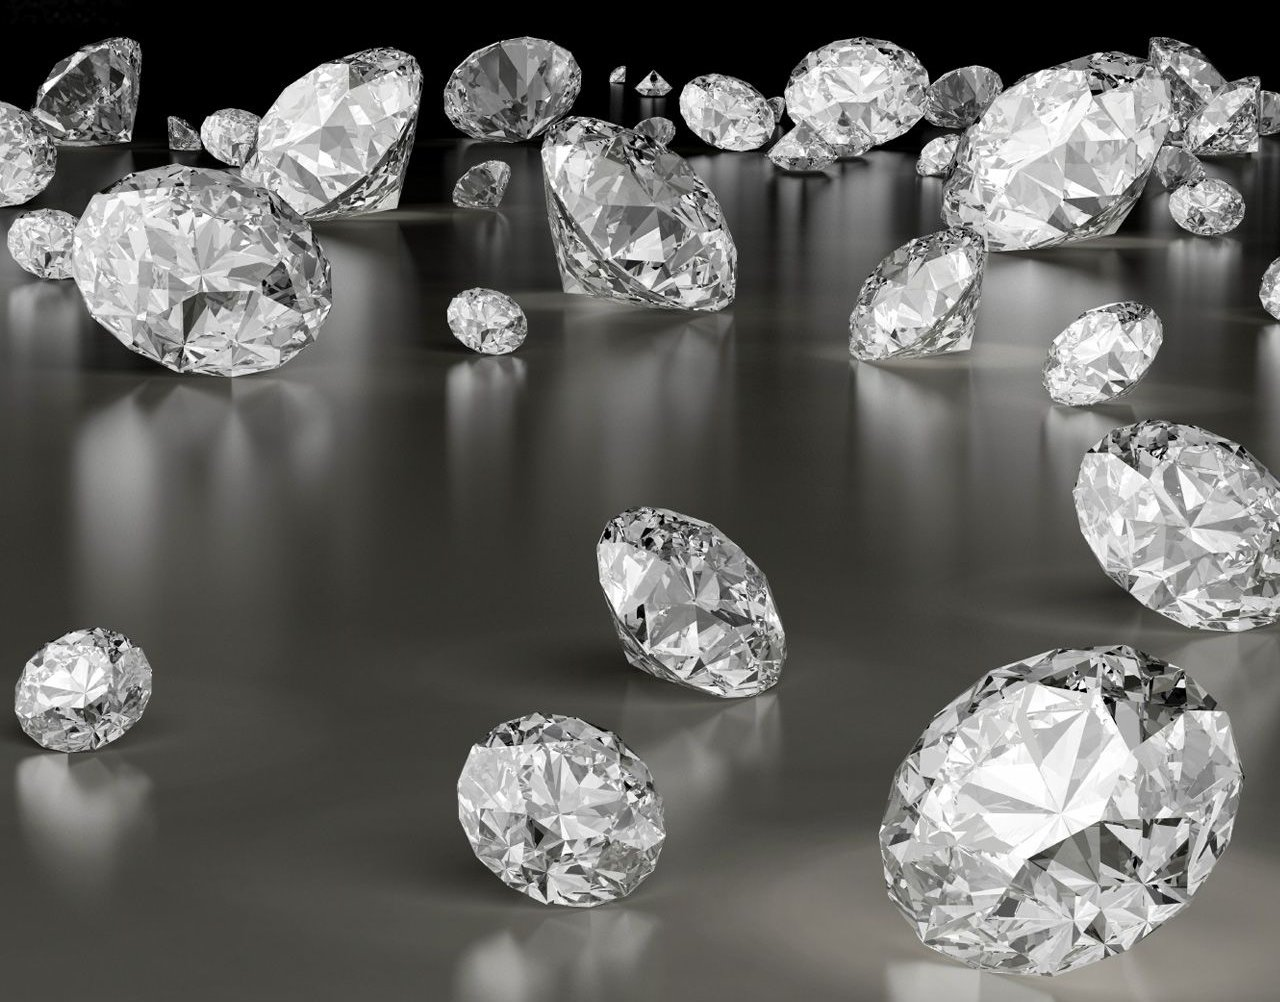
\includegraphics[width=1.13\paperwidth]{bkg}};
	\end{tikzpicture}
	
	\begin{minipage}[.2\textheight]{.4\textwidth}
    \begin{figure}[t]\flushleft
      \includegraphics[height=1cm]{ETHLogo}
    \end{figure}
	\end{minipage}\hfill
	\begin{minipage}[.2\textheight]{.4\textwidth}
    \begin{figure}[t]\flushright
      
\includegraphics[height=.9cm]{Logo_IPA_pos}
    \end{figure}
	\end{minipage}\vspace*{20pt}
	
	\begin{minipage}[.4\textheight]{\textwidth}
    \fig{.4}{\inserttitlegraphic}
	\end{minipage}
	
	\begin{block}{}
		\centering
		\vspace*{1pt}
		\usebeamerfont{title}\usebeamercolor[fg]{title}\textbf{\inserttitle}\\\vspace*{5pt}
		\usebeamerfont{subtitle}\insertsubtitle\\\vspace*{1pt}
	\end{block}
	\vspace*{10pt}
	\centering
	\color{black}
	\usebeamerfont{author}\textbf{\insertauthor}\par\vspace*{5pt}
	\usebeamerfont{date}\insertdate\par
}


\title[3D Pulse Height]{Pulse Height Analysis of 3D pCVD Diamond Detectors}
\subtitle{RD42 Meeting - Grenoble 2019}
\titlegraphic{3DTel1}
% END PREAMBEL

\begin{document}

{
	\setbeamertemplate{headline}{}
	\setbeamertemplate{footline}{}
	\begin{frame}[noframenumbering]
		\maketitle
	\end{frame}
}

{\setbeamertemplate{headline}{}
\begin{frame}{Table of Contents}%[allowframebreaks]
	\tableofcontents[hideallsubsections]   % [pausesections]
\end{frame}}


\section{Motivation}
%%%%%%%%%%%%%%%%%%%%%%%%%%%%%%%% FRAME 0 %%%%%%%%%%%%%%%%%%%%%%%%%%%%%%%%%%%%%%%%%%%%
\subsection{Diamond as Detector Material}
\begin{frame}{Diamond as Detector Material}

	\begin{itemize}\itemfill
		\item innermost tracking layers \ra highest radiation damage \orderof{\SI{}{\giga\hertz\per\centi\meter^2}}
% 		\item current detectors is designed to survive \SI{\sim12}{month} in High-Luminosity LHC
		\item \fat{\ra R\&D towards more radiation tolerant detector designs and/or materials}
	\end{itemize}\vspace*{2ex}
	
	\uncover<2->{
		\textbf{\underline{Diamond as Detector Material:}}\vspace*{5pt}
		\begin{itemize}\itemfill
			\item advantageous properties 
			\item \good{after \SI{1e16}{\ncm} the mean drift path in diamond larger than in silicon}
		\end{itemize}\vspace*{2ex}}
	
	\uncover<3->{
		\vspace*{5pt}\textbf{\underline{Work at ETH:}}\vspace*{5pt}
		\begin{itemize}
			\item investigate signals and radiation tolerance in various detector designs:\vspace*{5pt}
				\begin{itemize}\itemfill
							\alt<3>{
								\item Pad Detectors \ra whole diamond as single cell readout
								\item Pixel Detectors \ra diamond sensor on pixel readout chip
								\item 3D Pixel Detectors \ra 3D diamond detector on pixel readout chip}
								{
								\item \good{Pad Detectors} \ra this talk
								\item \fadeout{Pixel Detectors}
								\item \fadeout{3D Pixel Detectors}\vspace*{1.45pt}}
				\end{itemize}
		\end{itemize}}
		\pause[4]
		
\end{frame}

\section{3D Pixel Detector}
%%%%%%%%%%%%%%%%%%%%%%%%%%%%%%%% FRAME 0 %%%%%%%%%%%%%%%%%%%%%%%%%%%%%%%%%%%%%%%%%%%%
\subsection{3D Detectors}
\begin{frame}{Working Principle}

	\fig{.48}{3DConcept}
	
	\begin{itemize}\itemfill
		\item after large radiation fluence all detectors become trap limited
		\item bias and readout electrode inside detector material
		\item same thickness $D$ \ra same amount of induced charge \ra shorter drift distance $L$
		\item \good{increase collected charge in detectors with limited mean drift path (Schubweg)}
	\end{itemize}

\end{frame}

%%%%%%%%%%%%%%%%%%%%%%%%%%%%%%%% FRAME 1 %%%%%%%%%%%%%%%%%%%%%%%%%%%%%%%%%%%%%%%%%%%%
\begin{frame}{Bump Bonding}

	\subfigs{\subfig[.48][.1]{.3}{BondingSchemeCMS}[Bump bond schematics]}{\subfig[.44]{.4}{BBCMS1}[\SI{3x2}{} bump pads]}
	
	\begin{itemize}\itemfill
		\item electrodes (columns) drilled with femto-second laser
		\item connection to bias and readout with surface metallisation
		\item ganging of cells to match pixel pitch of readout-chip (ROC)
		\item small gap (\SI{\sim15}{\micro\meter}) to the surface to avoid a high voltage break-through 
	\end{itemize}

\end{frame}

\section{Reprocessing of II6-B6 in Fall 2019}
%%%%%%%%%%%%%%%%%%%%%%%%%%%%%%%%%%%%%% FRAME 0 %%%%%%%%%%%%%%%%%%%%%%%%%%%%%%%%%%%%%%%%%%%%%%%%
\begin{frame}{Reprocessing B6}

	\begin{itemize}\itemfill
		\item surface cleaning and RIE (Reactive Ion Etching) at OSU
		\item bias metallisation at OSU
		\item old mask was rotated...
	\end{itemize}
	
	\subfigs{\only<1-2>{\subfig{.5}{newmask}} \only<3>{\subfig{.5}{mask}}}{\only<1>{\subfig{.5}{B6m1}}\only<2->{\subfig{.5}{B6m2}}}
	
	
	\begin{itemize}
      \item new mask design including non drilled area for surface detector
      \item readout metallisation with new mask by Bert in Princeton
      \item bump-bonding very soon and then test at DESY 
    \end{itemize}

	
\end{frame}

\section{Setup at PSI}
%%%%%%%%%%%%%%%%%%%%%%%%%%%%%%%%%%%%%% FRAME 0 %%%%%%%%%%%%%%%%%%%%%%%%%%%%%%%%%%%%%%%%%%%%%%%%
\subsection{Telescope}
\begin{frame}{Pixel Telescope}

	\fig{.48}{3DTel}[modular ETH beam telescope in pixel configuration]
	
	\begin{itemize}\itemfill
		\item 4 tracking planes \ra trigger (fast-OR) \ra adjustable area (max \SI{8x7.8}{\milli\meter})
		\item up to 3 DUT planes (any digital pixel detector)
		\item scintillator for precise trigger timing \ra \orderof{\SI{1}{\nano\second}}
	\end{itemize}

\end{frame}
%%%%%%%%%%%%%%%%%%%%%%%%%%%%%%%%%%%%%% FRAME 1 %%%%%%%%%%%%%%%%%%%%%%%%%%%%%%%%%%%%%%%%%%%%%%%%
\subsection{Schematics}
\begin{frame}{Schematic Setup}

	\vspace*{-2ex}\fig{.55}{TelSchematicsDig}
	
	\begin{itemize}\itemfill
		\item independent telescope module for DUTs (dark green)
		\item scintillator \ra precise trigger timing of \orderof{\SI{1}{\nano\second}}
		\item Trigger Unit (TU) \ra strongly simplifying setup
		\item global trigger \ra (Plane 1 AND Plane 2) AND Scintillator
	\end{itemize}
	
\end{frame}

\section{Recent Results}
\subsection{Recent Results}
%%%%%%%%%%%%%%%%%%%%%%%%%%%%%%%%%%%%%% FRAME 0 %%%%%%%%%%%%%%%%%%%%%%%%%%%%%%%%%%%%%%%%%%%%%%%%
\begin{frame}{PSI - August 2017}

	\subfigs{\subfig{.5}[r]{PH1}}{\only<1>{\subfig{.5}[r]{EM1}}\only<2>{\subfig{.5}[r]{HE1}}}
	
	\begin{itemize}\itemfill
		\item<1-> pulse height looks OK, but ``pedestal'' of unknown origin (cannot be real)
		\begin{itemize}
			\item<1-> cannot be remeasured, since the ROC was exchanged 
		\end{itemize}
		\item<1-> Langau MPV: \SI{13500}{e}
		\item<1-> uniform efficiency
		\item<2> high efficiency of \SI{99.2\pm.1}{\%}
	\end{itemize}
	
\end{frame}

\section{Pulse Height Calibration}
%%%%%%%%%%%%%%%%%%%%%%%%%%%%%%%%%%%%%% FRAME 0 %%%%%%%%%%%%%%%%%%%%%%%%%%%%%%%%%%%%%%%%%%%%%%%%
\subsection{Pixel Unit Cell}
\begin{frame}{Pixel Unit Cell}

	\fig{.5}{PUC}
	
	\begin{itemize}\itemfill
		\item inject calibration signal ($\sim$\,vcal) through sensor into same circuit as real signals
		\item shaping, amplification, threshold check
		\item set amplification offset
		\item convert to \SI{8}{bit} adc value with adjustable scale \ra readout
	\end{itemize}
	
\end{frame}

%%%%%%%%%%%%%%%%%%%%%%%%%%%%%%%%%%%%%% FRAME 2 %%%%%%%%%%%%%%%%%%%%%%%%%%%%%%%%%%%%%%%%%%%%%%%%
\subsection{Trimming}
\begin{frame}{ADC Calibration}
    
    
    \subfigs{\only<1>{\subfig{.5}[r]{trim}[Threshold Map.]}\only<2>{\subfig{.5}[r]{s2020}}}{\only<1>{\subfig{.5}[r]{trimdist}[Threshold Distribution.]}\only<2>{\subfig{.5}[r]{s4040}}}

    \begin{itemize}\itemfill 
        \item<1-> trim all pixels to the same threshold
        \item<2> means pixel start to become efficient at the tuned threshold
    \end{itemize}

\end{frame}

%%%%%%%%%%%%%%%%%%%%%%%%%%%%%%%%%%%%%% FRAME 2 %%%%%%%%%%%%%%%%%%%%%%%%%%%%%%%%%%%%%%%%%%%%%%%%
\subsection{Tuning and Calibration}
\begin{frame}{ADC Calibration}
	
	
	\vspace*{-10pt}
	\only<1>{\fig[r]{.5}{AdcCal}[ADC calibration for single pixel.]}
	\only<2>{\fig[r]{.5}{AdcCalFit}[ADC calibration for single pixel with error function fit.]}

	\begin{itemize}\itemfill 
		\item<1-> measure adc values for calibration pulses with different vcal
		\item<1-> adc follows error function and saturates for high vcal
		\item<2> fit every pixel and save fit parameters
		\item<2> adjust adc offset and range with DACs of the chip
	\end{itemize}

\end{frame}


%%%%%%%%%%%%%%%%%%%%%%%%%%%%%%%%%%%%%% FRAME 2 %%%%%%%%%%%%%%%%%%%%%%%%%%%%%%%%%%%%%%%%%%%%%%%%
\begin{frame}{ADC Calibration - Temperature Dependence}
    
    \vspace*{-3ex}
    \fig[r]{.5}{tdep}[Read back VCAL inducing test-pulses with VCAL 200.]
    \vspace*{-2ex}

    \begin{itemize}\itemfill 
        \item readout chip heats up quite significantly while being in use
        \item adc calibration strongly temperature dependent 
        \item inducing test pulses with VCAL 200 at room temperature
        \begin{itemize}
          \item converting the measured ADC back to VCAL using the calibration
          \item VCAL only approaches the correct value after the chip reaches the correct temperature
        \end{itemize}
        \item \ra always perform calibration after heating up the chip!
    \end{itemize}

\end{frame}

%%%%%%%%%%%%%%%%%%%%%%%%%%%%%%%%%%%%%% FRAME 3 %%%%%%%%%%%%%%%%%%%%%%%%%%%%%%%%%%%%%%%%%%%%%%%%
\begin{frame}{Vcal Calibration (Silicon)}
	
	\def\d{.295}
	\only<1>{
		\begin{minipage}{.48\textwidth}
			\subfigs{\subfig{\d}{Zn}[Zn target.]}{\subfig{\d}{Mo}[Mo target.]}\vspace*{9.1ex}
		\end{minipage}
		\begin{minipage}{.48\textwidth}
			\subfigs{\subfig{\d}{Ag}[Ag target.]}{\subfig{\d}{Sn}[Sn target.]}\vspace*{9.1ex}
		\end{minipage}}
	\only<2>{\fig{.4}{VcalCal}[Vcal Calibration.]}
	\only<3>{\subfigs{\subfig{.439}[r]{VS}[Vcal slopes.]}{\subfig{.439}[r]{VO}[Vcal offsets.]}\vspace*{-2ex}}
	
	\begin{itemize}\itemfill 
		\item<1-> measure energy spectra of $K_{\alpha}$ lines of four metal targets using ADC-calibration
		\item<2-> linear dependence of energy [e] and vcal 
		\item<2-> fit $K_{\alpha}$ points with straight line (similar for each chip)
		\item<2-> impossible to do calibration with diamond (energy too low)
		\begin{itemize}
			\item<3-> use general values from silicon: $\z{e} = 46.5\cdot vcal$
		\end{itemize}
	\end{itemize}

\end{frame}

% \section{Analysis}
%%%%%%%%%%%%%%%%%%%%%%%%%%%%%%%%%%%%%% FRAME 0 %%%%%%%%%%%%%%%%%%%%%%%%%%%%%%%%%%%%%%%%%%%%%%%%
\subsection{Event Cuts}
\begin{frame}{Cuts}

	\nicetab{ll}{ \good{Cut} & \good{Excluded Events} 														\\\hline
	event range					& first minute of the run due to various beam conditions 	\\
	beam interruptions	& during rate changes of the beam due to beam interruption\\
	aligned 						& DUT and Telescope are not aligned (event-wise)					\\
	trigger phase				& Chip trigger timing is incorrect 												\\
	tracks							& not all telescope planes have exactly one cluster				\\
	chi2 (x/y)					& badly fit tracks (\SI{>50}{\%\, quantile})							\\
	track slope (x/y)		& large angles of the tracks (\SI{>2}{deg})								\\
	rhit								& large DUT residual (\SI{>100}{\milli\meter})						\\
	pixel mask					& noisy pixels																						\\
	fiducial						& not in selected (fiducial) area of the DUT							\\
	}[Analysis cut flow.]\vspace*{-6ex}
	
	\begin{minipage}{.6\textwidth}
		\begin{itemize}
			\item cuts applied in order of the table
			\item largest contribution usually by chi2, tracks and fiducial cuts
		\end{itemize}
	\end{minipage}\hfill
	\begin{minipage}{.3\textwidth}
		\fig[r]{.38}{CutPie}
	\end{minipage}



	
\end{frame}

\section{Results}
%%%%%%%%%%%%%%%%%%%%%%%%%%%%%%%%%%%%%% FRAME 0 %%%%%%%%%%%%%%%%%%%%%%%%%%%%%%%%%%%%%%%%%%%%%%%%
\subsection{Tracking Resolution}
\begin{frame}{Tracking Resolution}

	\subfigs{\subfig[.4]{.5}[r]{TR}}{\subfig[.55]{.33}{TelSchematics3}}
	
	\begin{itemize}\itemfill
		\item ROC = Plane
		\item resolution = width of the residual distribution at the plane under test
		\item can achieve \SI{\sim20}{\micro\meter} resolution at very low $\upchi^2$
		\item resolution at the front slightly better than in the back
		\begin{itemize}
			\item less multiple scattering
		\end{itemize}
% 		\item choose \SI{90}{\%} quantile to have a large number of events

	\end{itemize}
		
\end{frame}
%%%%%%%%%%%%%%%%%%%%%%%% FRAME 1 %%%%%%%%%%%%%%%%%%%%%%%%%%%%%%%
\subsection{Rate Measurements}
\begin{frame}{S129}

	\vspace*{-2ex}
	\only<1>{\fig[r]{.5}{S129EvoF}}
	\only<2>{\fig[r]{.5}{S129EvoZ}}
	\only<3>{\fig[r]{.5}{S129STD}}\vspace*{-1ex}
	
	\begin{itemize}\itemfill
		\item<1-> every point the mean of a whole rate scan
		\item<1-> very high points have no attenuator
		\item<1-> first two points have a change in amplifier
		\item<2-> most points very stable over time but some fluctuate (maybe DRS4 issue)
		\item<3-> standard deviation in general below \SI{.5}{\%}
	\end{itemize}

\end{frame}
%%%%%%%%%%%%%%%%%%%%%%%% FRAME 1 %%%%%%%%%%%%%%%%%%%%%%%%%%%%%%%
\begin{frame}{B2 Rate Scans}

	\begin{minipage}[c][.7\textheight]{.34\textwidth}
		\begin{itemize}\itemfill
			\item after irradiation pulse height is very stable
			\item maximum irradiation: \SI{8e15}{\ncm}
			\item little drop for high rates at high irradiations 
			\item \ra due to decreasing signals one cut is working less efficient
			\item<2> positive and negative bias agree very well
		\end{itemize}
	\end{minipage}\hfill
	\begin{minipage}{.63\textwidth}
		\only<1>{\fig{.8}{B2All}}
		\only<2>{\fig{.8}{B2AllP}}
	\end{minipage}
	
\end{frame}
%%%%%%%%%%%%%%%%%%%%%%%% FRAME 1 %%%%%%%%%%%%%%%%%%%%%%%%%%%%%%%
\begin{frame}{B2 Pulse Height Evolution}

	\vspace*{-3ex}
	\fig[r]{.6}{B2M}

	\def\d{\hspace*{1ex}}
	\hspace*{17ex} 0 \d\ra\d \SI{5e14}{} \d\ra\d \SI{1e15}{} \d\ra\d \SI{2e15}{} \ra \SI{4e15}{} \ra \SI{8e15}{\ncm}\vspace*{3ex}
	\begin{itemize}\itemfill
		\item absolute pulse height decreases exponentially
		\item SNR at highest irradiation only 2/1 \ra prevents next step with this amplifier \ra use new OSU amp?
	\end{itemize}

\end{frame}
%%%%%%%%%%%%%%%%%%%%%%%% FRAME 3 %%%%%%%%%%%%%%%%%%%%%%%%%%%%%%%
\begin{frame}{Fix Rate Dependence}

	\subfigs{\subfig{.5}[r]{PHB}[First measurement]}{\subfig{.5}[r]{PHB2}[After reprocessing]}
	
	\begin{itemize}\itemfill
		\item less than \SI{20}{\%} of the tested diamonds show rate dependence \SI{>10}{\%}
		\item very large rate dependence at the first measurement (\SI{>90}{\%})
		\item after reprocessing and surface cleaning with RIE very stable behaviour (\SI{\sim2}{\%})
		\item feasible to ``fix'' bad diamonds
	\end{itemize}

\end{frame}


\section{Conclusion}
\begin{frame}{Conclusion}

	\begin{minipage}[c][4cm]{\textwidth}
		\begin{itemize}
			\itemfill
			\item many different measurement of both 3D diamond detectors
			\begin{itemize}
				\item start analyse more data!\vspace*{2ex}
			\end{itemize}
			\item X-ray pulse height calibration can hardly be performed on diamond
			\begin{itemize}
				\item need to use estimate from silicon\vspace*{2ex}
			\end{itemize}
			\item adc calibration is very temperature dependent 
			\begin{itemize}
				\item need to perform calibration after chip heated up
			\end{itemize}
			\item pulse height can significantly fluctuate below threshold                    
			\item pulse height results on single planes very reasonable without distributions below threshold
		\end{itemize}
	\end{minipage}
	
\end{frame}

\setbeamertemplate{footline}{}
\setbeamertemplate{headline}{}
\begin{frame}[noframenumbering]

	\begin{tikzpicture}[remember picture,overlay]
		\node[at=(current page.center)] {
			
\includegraphics[width=.7\paperwidth]{delfin2.pdf}};
	\end{tikzpicture}
	
\end{frame}
 % FINAL PAGE
\section*{Backup}
%%%%%%%%%%%%%%%%%%%%%%%%%%%%%%%%%%%%%% FRAME 1 %%%%%%%%%%%%%%%%%%%%%%%%%%%%%%%%%%%%%%%%%%%%%%%%
\subsection{Timing Correction}
\begin{frame}[noframenumbering]{Ringbuffer}

	\subfigs{\subfig{.5}{ringbuffer}[Ringbuffer]}{\subfig{.5}[r]{TCAL}[Length of memory cells.]}
	
	\begin{itemize}\itemfill
		\item analogue signals of the diamonds constantly digitised and saved in ringbuffer
		\item overwrite old data once again at first cell
		\item once triggered data is saved starting from the current cell \ra trigger cell
		\item measure the length the of memory cells of the DRS4 (before every beam test)
		\item record trigger cell for every event
	\end{itemize}

\end{frame}
%%%%%%%%%%%%%%%%%%%%%%%%%%%%%%%%%%%%%% FRAME 2 %%%%%%%%%%%%%%%%%%%%%%%%%%%%%%%%%%%%%%%%%%%%%%%%
\begin{frame}[noframenumbering]{Peak Position}

	\subfigs{\subfig{.5}[r]{PeakPos}[no correction]}{\subfig{.5}[r]{PeakPos10}[with correction]}
	
	\begin{itemize}\itemfill
		\item timing of the signals should be fixed and determined by the scintillator
		\item non-corrected peak time distribution resembles cell size distribution
		\item correcting for the different cell sizes \ra strong improvement in timing
	\end{itemize}

\end{frame}
%%%%%%%%%%%%%%%%%%%%%%%%%%%%%%%%%%%%%% FRAME 3 %%%%%%%%%%%%%%%%%%%%%%%%%%%%%%%%%%%%%%%%%%%%%%%%
\begin{frame}[noframenumbering]{Fine Correction}

	\subfigs{\subfig{.5}[r]{PeakTC}[Dependence on trigger cell.]}{\subfig{.5}[r]{FineCorr}[fine correction]}
	
	\begin{itemize}\itemfill
		\item after drs4 time correction \ra still timing depends periodically on the trigger cell (why?)
		\item fit with periodic function with known period 
	\end{itemize}

\end{frame}
%%%%%%%%%%%%%%%%%%%%%%%%%%%%%%%%%%%%%% FRAME 4 %%%%%%%%%%%%%%%%%%%%%%%%%%%%%%%%%%%%%%%%%%%%%%%%
\begin{frame}[noframenumbering]{Timing Correction + Cut}

	\subfigs{\subfig{.5}[r]{TCor}[All corrections]}{\subfig{.5}[r]{TCorFit}[Timing cut]}
	
	\begin{itemize}\itemfill
		\item achieve \SI{\sim500}{\pico\second} timing resolution
		\item exclude signals outside \SI{3}{\sigma}) of this distribution
		\begin{itemize}
			\item wrong timing means something went wrong in the data-taking or the waveform is bad
		\end{itemize}
	\end{itemize}

\end{frame}
%%%%%%%%%%%%%%%%%%%%%%%%%%%%%%%%%%%%%% FRAME 0 %%%%%%%%%%%%%%%%%%%%%%%%%%%%%%%%%%%%%%%%%%%%%%%%
\subsection{Bucket Cut}
\begin{frame}[noframenumbering]{Origin}

	\only<1>{\fig{.5}{Bucket}}
	\only<2>{\fig{.5}{bucketwf}}
	
	\begin{itemize}\itemfill
		\item bunch spacing of PSI (\SI{19.7}{\nano\second}) small than clock cycle of fast-OR (\SI{25}{\nano\second})
		\item scintillator area \SI{\sim10}{times} larger than active trigger area
		\item within one clock cycle of \SI{25}{\nano\second}:
		\begin{itemize}
			\item \bad{one particle only hits the scintillator}
			\item \good{second particle hits the telescope and the diamond}
		\end{itemize}
		\item \ra no signal in signal region!
	\end{itemize}
	
\end{frame}
%%%%%%%%%%%%%%%%%%%%%%%%%%%%%%%%%%%%%% FRAME 1 %%%%%%%%%%%%%%%%%%%%%%%%%%%%%%%%%%%%%%%%%%%%%%%%
\begin{frame}[noframenumbering]{Bucket Pedestal}

	\fig[r]{.5}{Bucket1}
	
	\begin{itemize}\itemfill
		\item flat lines only when the highest peak is in the bunch after the trigger
	\end{itemize}
		
\end{frame}
%%%%%%%%%%%%%%%%%%%%%%%%%%%%%%%%%%%%%% FRAME 2 %%%%%%%%%%%%%%%%%%%%%%%%%%%%%%%%%%%%%%%%%%%%%%%%
\begin{frame}[noframenumbering]{Bucket Cut}

	\vspace*{-15pt}\fig[r]{.7}{Bucket2}
	
	\begin{itemize}\itemfill
		\item fit signal distribution when signal in the bunch after the trigger is higher
		\item signal and background well separated
		\item shift threshold and minimise the error on the signal
	\end{itemize}
		
\end{frame}%%%%%%%%%%%%%%%%%%%%%%%%%%%%%%%%%%%%%% FRAME 0 %%%%%%%%%%%%%%%%%%%%%%%%%%%%%%%%%%%%%%%%%%%%%%%%
\subsection{Event Selection}
\begin{frame}[noframenumbering]{Saturated}

	\fig[r]{.4}{sat}

	\begin{itemize}\itemfill
		\item DRS4 signal range: [-500, +500]\, mV
		\item exclude saturated waveforms \ra full pulse height information lost
		\item main source should be protons
		\item 17/200000 events in example above
	\end{itemize}
	
\end{frame}
%%%%%%%%%%%%%%%%%%%%%%%%%%%%%%%%%%%%%% FRAME 1 %%%%%%%%%%%%%%%%%%%%%%%%%%%%%%%%%%%%%%%%%%%%%%%%
\begin{frame}[noframenumbering]{Pulser}

	\only<1>{\fig[r]{.4}{PW}}
	\only<2>{\fig[r]{.4}{pul}}

	\begin{itemize}\itemfill
		\item<1-> use pulser as a reference signal
		\item<1-> tag pulser events by extra channel of the DRS4
		\item<2-> exclude these event since they don't have a diamond signal
		\item<2-> use for pulser analysis to compare to diamond signal
	\end{itemize}
	
\end{frame}
%%%%%%%%%%%%%%%%%%%%%%%%%%%%%%%%%%%%%% FRAME 2 %%%%%%%%%%%%%%%%%%%%%%%%%%%%%%%%%%%%%%%%%%%%%%%%
\begin{frame}[noframenumbering]{Event Range}
	
	\vspace*{-10pt}\fig[r]{.5}{ER}

	\begin{itemize}\itemfill
		\item until October 2015 \ra beam shutter opened after run was started
		\begin{itemize}
			\item unstable conditions
			\item exclude first five minutes of the run\vspace*{5pt}
		\end{itemize}
		\item past October 2015 exclude first minute as safety margin
		\begin{itemize}
			\item sometimes small adjustments made (e.g. collimator changed too late)
		\end{itemize}

	\end{itemize}
	
\end{frame}
%%%%%%%%%%%%%%%%%%%%%%%%%%%%%%%%%%%%%% FRAME 3 %%%%%%%%%%%%%%%%%%%%%%%%%%%%%%%%%%%%%%%%%%%%%%%%
\begin{frame}[noframenumbering]{Beam Interruption}
	
	\only<1>{\fig[r]{.4}{FP}}
	\only<2>{\fig[r]{.4}{FP1}}

	\begin{itemize}\itemfill
		\item<1-> usually short beam interruption every \SI{5}{\minute} at PSI + other interruption
		\item<2-> particle rate slowly ramps up after interruption
		\item<2-> exclude events when rate drops less than \SI{40}{\%} + \SI{5}{\second} before
		\item<2->  until rate is larger than \SI{40}{\%} + \SI{20}{\second} after this
		\item<2-> let pulse height adjust after beam interruption (safety margin)
	\end{itemize}
	
\end{frame}
%%%%%%%%%%%%%%%%%%%%%%%%%%%%%%%%%%%%%% FRAME 4 %%%%%%%%%%%%%%%%%%%%%%%%%%%%%%%%%%%%%%%%%%%%%%%%
\begin{frame}[noframenumbering]{Tracks}
	
	\fig[r]{.6}{OCs}

	\begin{itemize}\itemfill
		\item only use events with exactly one track
		\item require one and only one cluster per plane
	\end{itemize}
	
\end{frame}
%%%%%%%%%%%%%%%%%%%%%%%%%%%%%%%%%%%%%% FRAME 5 %%%%%%%%%%%%%%%%%%%%%%%%%%%%%%%%%%%%%%%%%%%%%%%%
\begin{frame}[noframenumbering]{Pedestal Sigma}
	
	\subfigs{\subfig{.5}[r]{PD}}{\subfig{.5}[r]{PDL}}

	\begin{itemize}\itemfill
		\item exclude pedestals outside the 3 sigma region
		\item baseline shifts
		\item bad waveforms
	\end{itemize}
	
\end{frame}
%%%%%%%%%%%%%%%%%%%%%%%%%%%%%%%%%%%%%% FRAME 9 %%%%%%%%%%%%%%%%%%%%%%%%%%%%%%%%%%%%%%%%%%%%%%%%
\begin{frame}[noframenumbering]{$\upchi^2$}

	\subfigs{\subfig{.5}[r]{ChiX}}{\subfig{.5}[r]{ChiY}}
	
	\begin{itemize}\itemfill
		\item exclude the bad tracks
	\end{itemize}
		
\end{frame}
%%%%%%%%%%%%%%%%%%%%%%%%%%%%%%%%%%%%%% FRAME 12 %%%%%%%%%%%%%%%%%%%%%%%%%%%%%%%%%%%%%%%%%%%%%%%
\begin{frame}[noframenumbering]{Tracking Angle}

	\only<1>{\subfigs{\subfig{.5}[r]{TAX1}}{\subfig{.5}[r]{TAY1}}}
	\only<2>{\subfigs{\subfig{.5}[r]{TAX}}{\subfig{.5}[r]{TAY}}}
	
	\begin{itemize}\itemfill
		\item only accept tracks with small angles
		\item<2-> angle only very slightly changes with rate
	\end{itemize}
		
\end{frame}
%%%%%%%%%%%%%%%%%%%%%%%%%%%%%%%%%%%%%% FRAME 13 %%%%%%%%%%%%%%%%%%%%%%%%%%%%%%%%%%%%%%%%%%%%%%%
\begin{frame}[noframenumbering]{Fiducial Cut}

	\subfigs{\subfig{.5}[r]{fid}}{\subfig{.5}[r]{fid1}}
	
	\begin{itemize}\itemfill
		\item select area of the diamond
		\item find first and last bin when signal drops lower than \SI{93}{\%} of the maximum value
		\item interpolate with the adjacent bins when threshold is exactly hit
		\item adjust manually if it fails or still pedestal left
	\end{itemize}
		
\end{frame}


\end{document} % DOCUMENT END
